\documentclass{article}

% Language setting
% Replace `english' with e.g. `spanish' to change the document language
\usepackage[english]{babel}

% Set page size and margins
% Replace `letterpaper' with `a4paper' for UK/EU standard size
\usepackage[letterpaper,top=2cm,bottom=2cm,left=3cm,right=3cm,marginparwidth=1.75cm]{geometry}

% Useful packages
\usepackage{amsmath}
\usepackage{graphicx}
\usepackage[colorlinks=true, allcolors=blue]{hyperref}
\usepackage{float}

\title{CS460: Assignment 1}
\author{Arya Shetty || Damon Lin}
\begin{document}
\maketitle

\section{Validating Rotations}

Important note, to run on the iLab computers just use the python environment: \\
\$ source /common/system/venv/python310/bin/activate \\
The rest of the libraries were just numpy and matplotlib.\\
Within the program, the epsilon parameter was implemented as tolerance to check that the answer was within a given numerical precision. For example, in the first function, \texttt{check\_SOn(m)}, if the determinant of the matrix minus one is greater than the epsilon numerical precision, then the matrix does not belong in the Special Orthogonal group.

\subsection{\texttt{check\_SOn(m)}}

This function checks whether the input matrix \texttt{m} satisfies the conditions for Special Orthogonal Groups. The conditions to check for include: the input matrix is a square, the matrix is orthogonal, and the determinant of the matrix is equal to 1. In this context, epsilon checks whether the determinant is within its numerical precision.

\subsection{\texttt{check\_quaternion(v)}}

This function checks whether the input vector \texttt{v} satisfies the quaternion conditions. The two conditions for a vector to be in Quaternions are: the vector is a unit vector and the vector is of length four. Therefore, the function first checks that the vector is of length four and then verifies whether the vector is a unit vector. The implementation to check the latter utilizes the \texttt{nn.allclose()} function comparing the normalized vector \texttt{v} with a unit vector while ensuring that the range is within the epsilon numerical precision.

\subsection{\texttt{check\_SEn(m)}}

The function \texttt{check\_SEn(m)} verifies that the input matrix \texttt{m} satisfies the conditions to belong in the Special Euclidean Groups. Thus, such a matrix must satisfy the following conditions:
\begin{itemize}
    \item[1.] The matrix is 2D.
    \item[2.] The rotation matrix within the matrix is either for 2D or 3D rotation.
    \item[3.] The rotation matrix must belong to the Special Orthogonal group.
    \item[4.] The bottom row must have $[0, 0, \ldots, 1]$.
\end{itemize}

\subsection{\texttt{correct\_SOn(m)}}

The function first checks if the matrix is orthogonal by testing $M\cdot M^{T}$. If it's not orthogonal, it corrects the matrix so it is closer to an orthogonal one. Then, it checks if the determinant is close to 1. If not, it corrects the matrix so that the determinant becomes 1. This approach ensures that the corrected matrix is orthogonal and has a determinant of 1, ensuring membership in the Special Orthogonal Groups.

\subsection{\texttt{correct\_quaternion(v)}}

The function first checks that the input is a valid 4-dimensional vector.  Then, it verifies whether the vector is a unit quaternion (norm of 1). If the vector is not a unit quaternion, the function normalizes it to make it one. The goal of the function is to ensure that the vector \texttt{v} represents a valid unit quaternion, correcting it if necessary while keeping it as close as possible to the original vector.

\subsection{\texttt{correct\_SEn(m)}}

Similar to the implementation of c\texttt{check\_SEn(m)}, this correction function checks to see whether the rotation matrix within matrix \texttt{m} is part of the Special Orthogonal group. If the rotation matrix is part of that group, the function checks the bottom row of the matrix and fixes it if there are any problems. On the other hand, if the rotation matrix is not part of the group, the function applies the \texttt{correct\_SOn(m)} function onto the rotation matrix. After, the program goes through the same steps as before, correcting the bottom row of the matrix if there are issues.

\section{Uniform Random Rotations}

\subsection{\texttt{random\_rotation\_matrix(naive)}}

This function generates a random rotation matrix, in two different ways. The naive approach picks three random Euler angles (using np.random.uniform) and creates the three rotation matrices for each axis based on these angles. Finally, it multiplies all the matrices to get the final rotation matrix. Since they started as rotation matrices it already meets the SO(n) conditions. The non-naive approach involves an algorithm from the paper. Here the rotation matrix won't always meet the conditions. However, the method allows for a more random choice of rotation matrices as shown by the images below. The main reason is that the Euler angles have a bias in sampling random angles, while the other approach uses a random vector to create the reflection matrix and cover more of the space. The images below are made with 1000 randomly generated rotation matrices.

\begin{figure} [H]
    \centering
    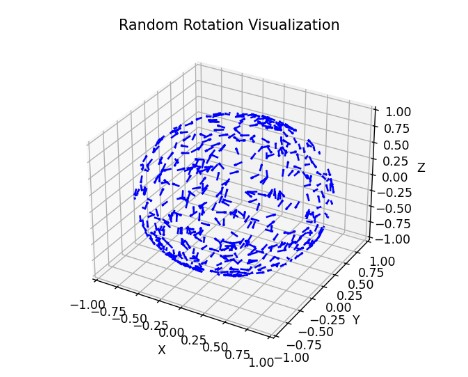
\includegraphics[width=0.5\linewidth]{latex_media/Random Rotation Visualization naive.jpg}
    \caption{Random Rotation Visualization naive}
    \label{fig:1}
\end{figure}

\begin{figure} [H]
    \centering
    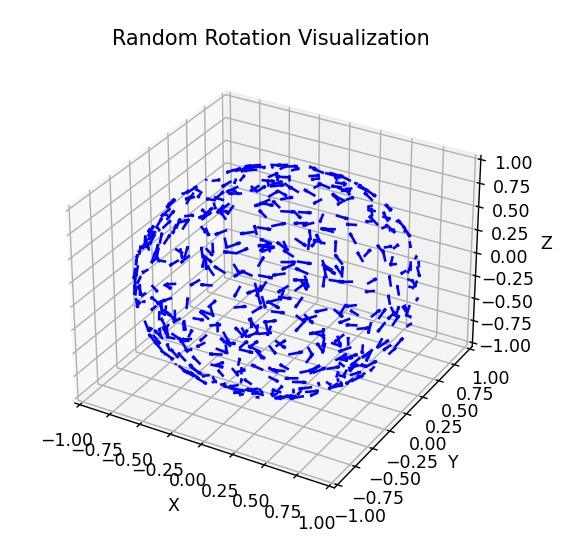
\includegraphics[width=0.5\linewidth]{latex_media/Random Rotation Visualization non-naive.jpg}
    \caption{Random Rotation Visualization non-naive}
    \label{fig:2}
\end{figure}


\subsection{\texttt{random\_quaternion(naive)}}

This function builds off the previous function \texttt{random\_rotation\_matrix(naive)}. As such, for the naive implementation, after the Euler angles are generated and the rotation matrices are calculated, the rotation matrices are converted to a quaternion. For the non-naive part, the same train of thought is applied once more wherein a new quaternion is produced until it satisfies \texttt{check\_quaternion(v)}. In the same fashion, the images come from 500 randomly generated quaternions.

\begin{figure} [H]
    \centering
    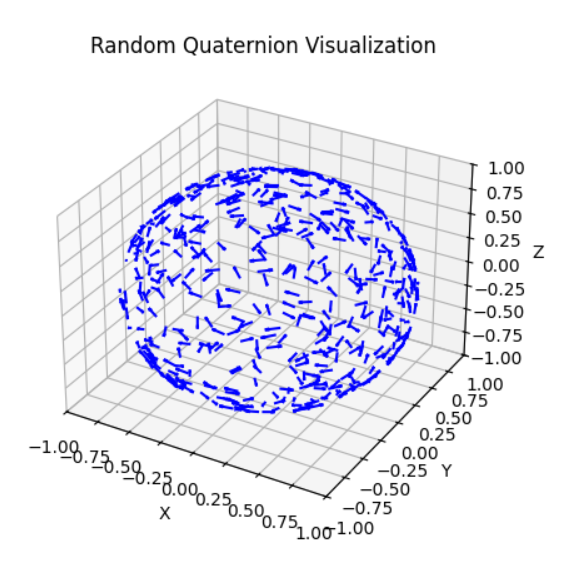
\includegraphics[width=0.5\linewidth]{latex_media/component_2_random_q_naive.png}
    \caption{Random Quaternion Visualization naive}
\end{figure}

\begin{figure} [H]
    \centering
    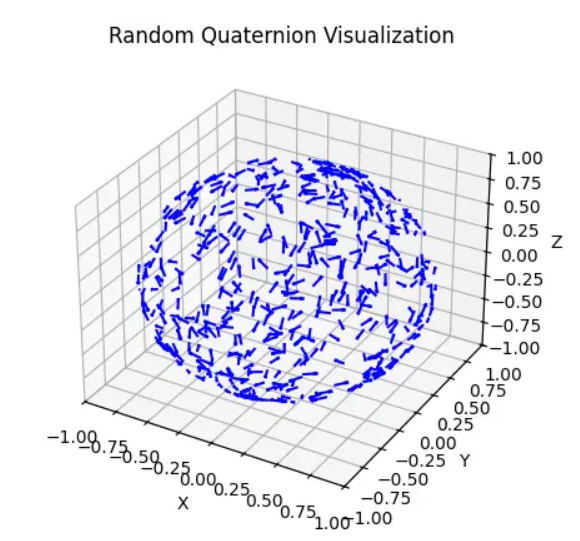
\includegraphics[width=0.5\linewidth]{latex_media/component_2_random_q_nonnaive.png}
    \caption{Random Quaternion Visualization non-naive}
\end{figure}
\section{Rigid body in motion}


\subsection{\texttt{interpolate\_rigid\_body(start\_pose, goal\_pose)}}

The idea for this function is to have the robot traverse from its start pose labeled in tuple form of (x, y, theta) to some goal. In this case, I predefined the amount of steps I want to take towards the goal, adjusting this will yield more or less poses depending on how smooth of a translation you want. The x and y translation is easily done using linspace to divide the distance equally. The rotation is the hard part since there could be singularities depending on whether the goal theta was greater than pi since a simple algorithm to divide the distance wouldn't work as it can take a longer path to reach the final angle (ex. going from 0 to 200 degrees, the faster way would be to go in the negative direction). So to account for this we used a SLERP design, spherical linear interpolation. The first step was getting the rotation matrices for the start and goal angles. Then we get the relative rotation matrix by multiplying the goal rotation matrix with the inverse of the start rotation matrix, which gives how much we should rotate without need of start orientation. Then you can get the angle from the matrix (use arctan) and iterate through it to get the poses for the path. To get the angle for the path you get the rotation matrix for the iterated angle and multiply it with the start pose, to get one of the iterations of the interpolated matrix. Then extract the angle like last time to use the interpolated theta for the pose. The following images are for start\_pose =  (0, 0, 0) and end\_pose = (4, 5, np.pi/2). The box's bottom left point is in line with the pose.

\begin{figure} [H]
    \centering
    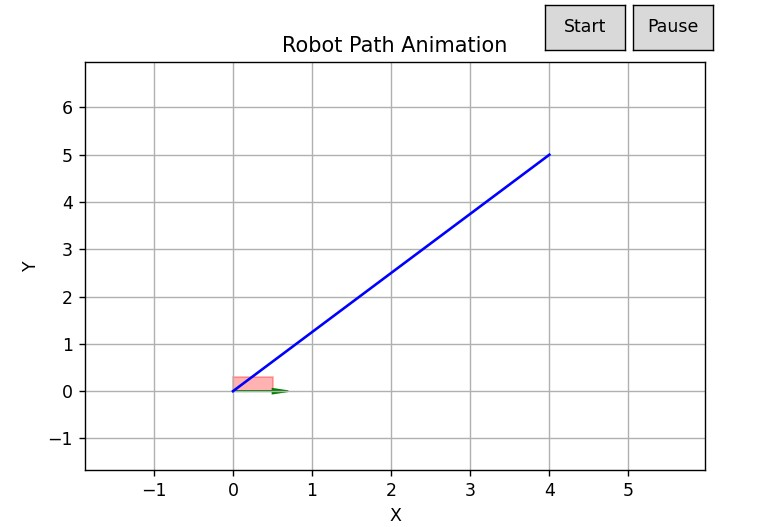
\includegraphics[width=0.5\linewidth]{latex_media/start of robot path anim.jpg}
    \caption{Start of robot path animation}
    \label{fig:3}
\end{figure}

\begin{figure} [H]
    \centering
    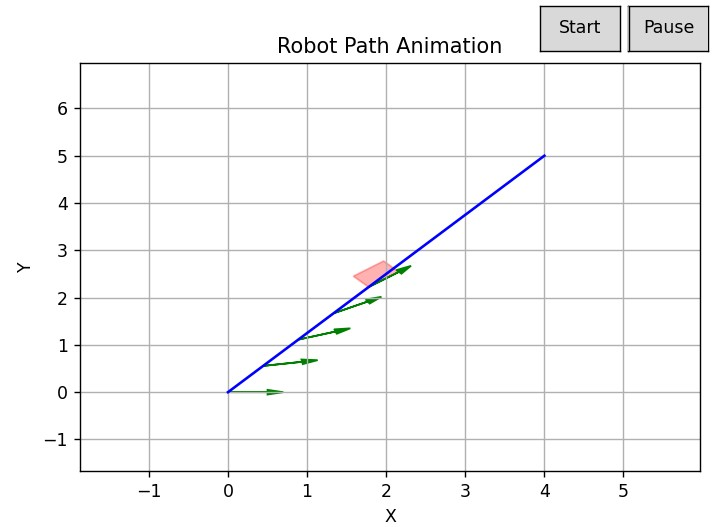
\includegraphics[width=0.5\linewidth]{latex_media/middle of robot path anim.jpg}
    \caption{Middle of robot path animation}
    \label{fig:4}
\end{figure}

\begin{figure} [H]
    \centering
    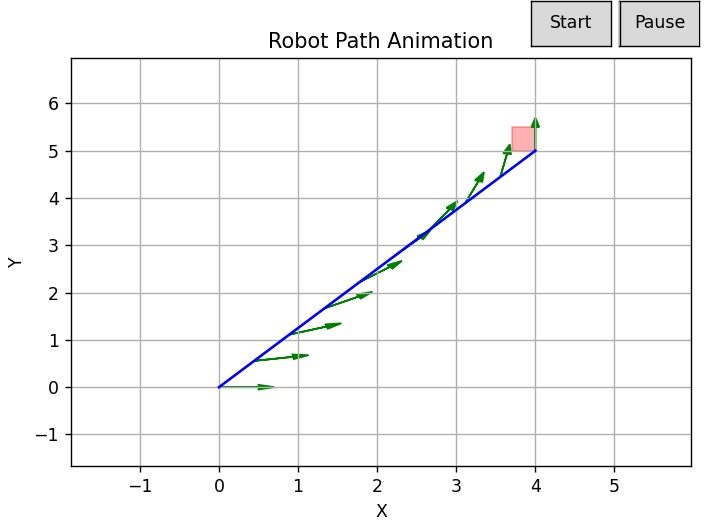
\includegraphics[width=0.5\linewidth]{latex_media/end of robot path anim.jpg}
    \caption{End of robot path animation}
    \label{fig:5}
\end{figure}

\subsection{\texttt{forward\_propagate\_rigid\_body(start\_pose, plan)}}

For this function we need to create a path based on the plan the robot is given, which is a sequence of tuples (velocity, duration). First we make sure the start pose is in bounds. Then we iterate through the plan, getting the Vx, Vy, Vtheta, and duration. Then multiply the velocities and duration to get the distance and angle traveled. Next, we applied the rotation matrix to get into the world frame and get the x and y the box ends up at. Finally the angle we just add to the box's theta currently. The images below are for plan = [
     (1, 1, np.radians(45), 1), 
     (1, 0, np.radians(45), 2),   
     (1, 0, 0, 2),
     (1, 0, np.radians(45), 1),
     (1, 0, 0, 2)   
     ]

\begin{figure} [H]
    \centering
    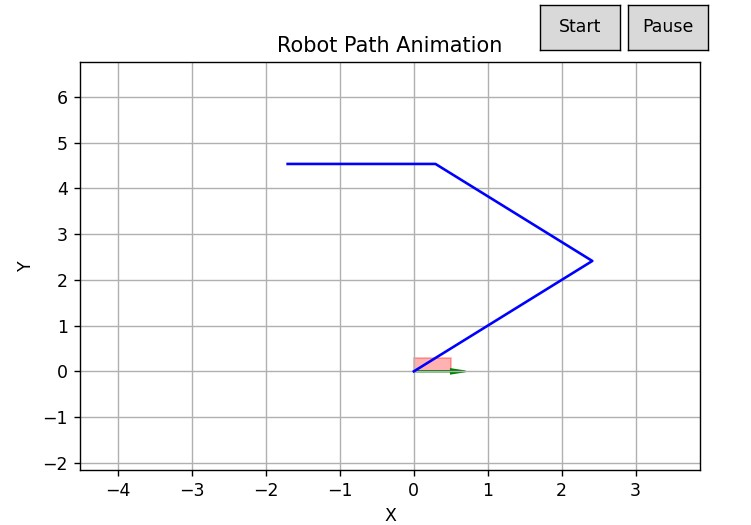
\includegraphics[width=0.5\linewidth]{latex_media/start of forward propagate anim.jpg}
    \caption{start of forward propagate anim}
    \label{fig:6}
\end{figure}

\begin{figure} [H]
    \centering
    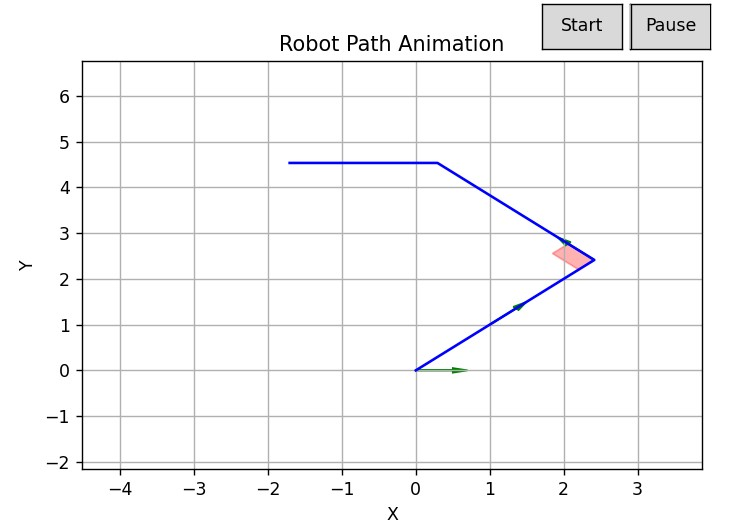
\includegraphics[width=0.5\linewidth]{latex_media/middle of forward propagate anim.jpg}
    \caption{middle of forward propagate anim}
    \label{fig:7}
\end{figure}

\begin{figure} [H]
    \centering
    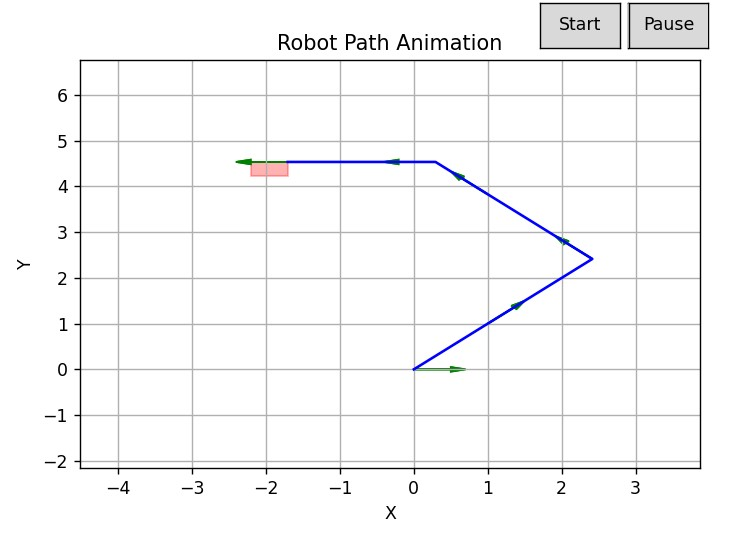
\includegraphics[width=0.5\linewidth]{latex_media/end of forward propagate anim.jpg}
    \caption{end of forward propagate anim}
    \label{fig:8}
\end{figure}

\subsection{\texttt{visualize\_path(path)}}


This function was used to animate and view the paths generated from each of the functions. It uses Matplotlib's library to help. We used the patches import to create the box for the robot based on the dimensions given and updated the position of each frame with the next pose. We also rotated it based on the theta and added start and pause buttons to look at each step. Then for each pose in the path the box's center is adjusted based on the x and y, and robot dimensions, and it is rotated to the theta. (Gifs in folder)

\section{Movement of an Arm}


\subsection{\texttt{interpolate\_arm(start, goal)}}

This function is similar to the rigid body's movement except with two arm links. Here we apply the technique of unwrapping the angle to avoid singularities we can get when traversing to the goal angle. This time we need to apply it twice for each arm. Once we get the next angles for each arm, we want to get poses for the path of each arm. In this case, we will be using four tuples to animate the robot, the joint of the first arm, the link of the first arm, the joint of the second arm, and the link of the second arm. We get this by using forward kinematics, which calculates the orientation with our angles. So we find the first joint by using the angle of the arm, and that's done with simple geometry as we line the base with the origin. The second arm is similar but we add the first arm's coordinate and theta since it is relative to the arm. Then the function returns four tuples. The first is the center point of the first arm which is L1 which is just the length divided by 2. The second tuple is the midpoint of the second arm or L2. Then the final two tuples are the end effectors of each arm. Finally, we return the path of these poses at the end and go to the next iteration. The images below are for start =  (np.radians(0), np.radians(45)) and goal = (np.radians(135), 0).

\begin{figure} [H]
    \centering
    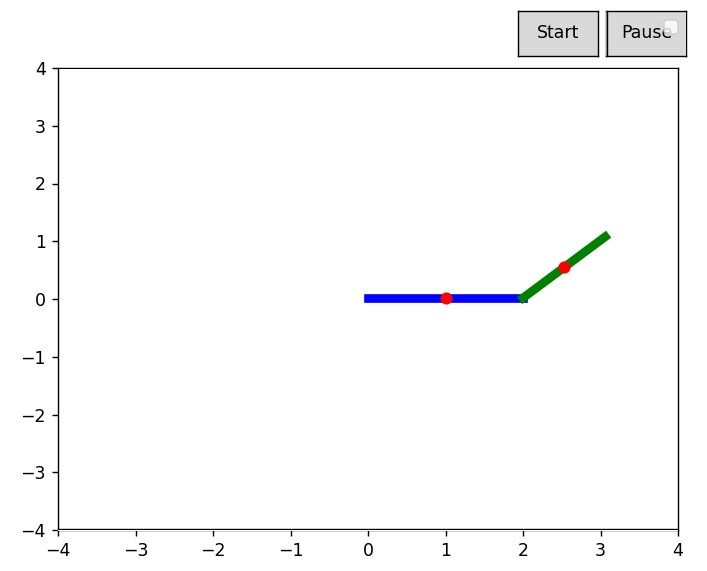
\includegraphics[width=0.5\linewidth]{latex_media/start of arm anim.jpg}
    \caption{start of arm anim}
    \label{fig:9}
\end{figure}

\begin{figure} [H]
    \centering
    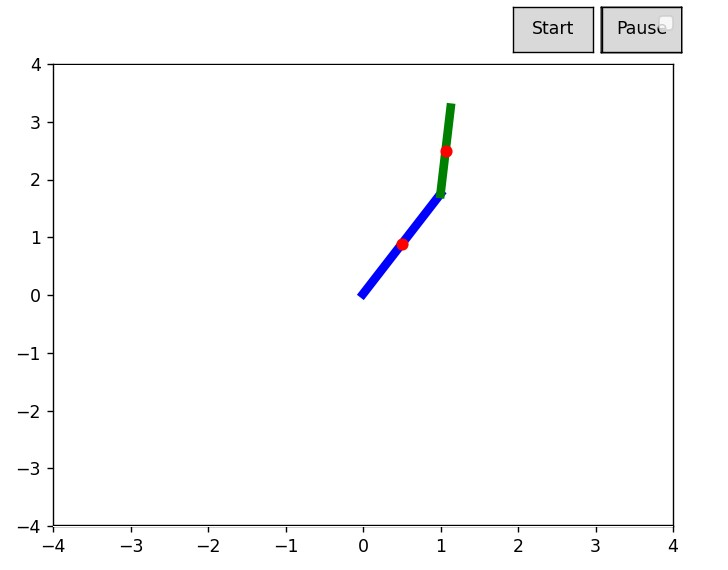
\includegraphics[width=0.5\linewidth]{latex_media/middle of arm anim.jpg}
    \caption{middle of arm anim}
    \label{fig:10}
\end{figure}

\begin{figure} [H]
    \centering
    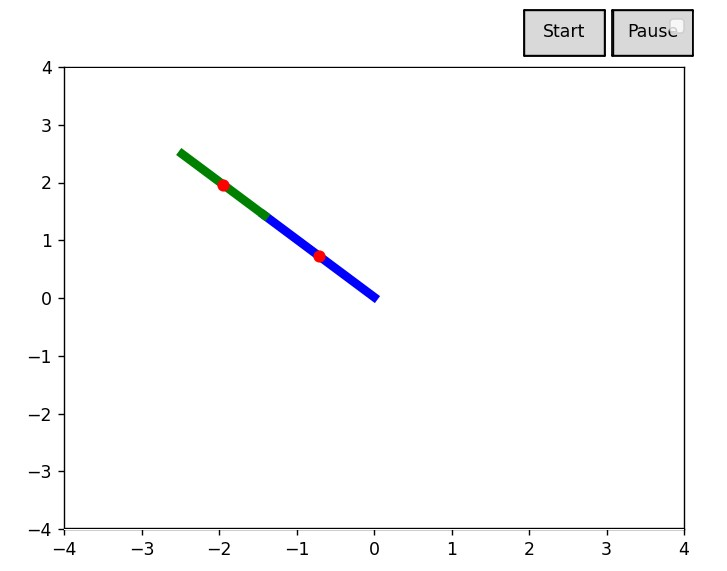
\includegraphics[width=0.5\linewidth]{latex_media/end of arm anim.jpg}
    \caption{end of arm anim}
    \label{fig:11}
\end{figure}

\subsection{\texttt{forward\_propagate\_arm(start\_pose, plan)}}

This function also returns a path but takes in a plan of tuples (velocity, duration) for the robot arms to move. Here We multiply the velocity for one arm to move by the duration to get the amount the theta should move based on the start pose. We then use the forward kinematics again to calculate the poses. The images below are for plan = [((0, np.radians(30)), 2), ((np.radians(45), 0), 1), ((np.radians(60), 0), 1)].

\begin{figure} [H]
    \centering
    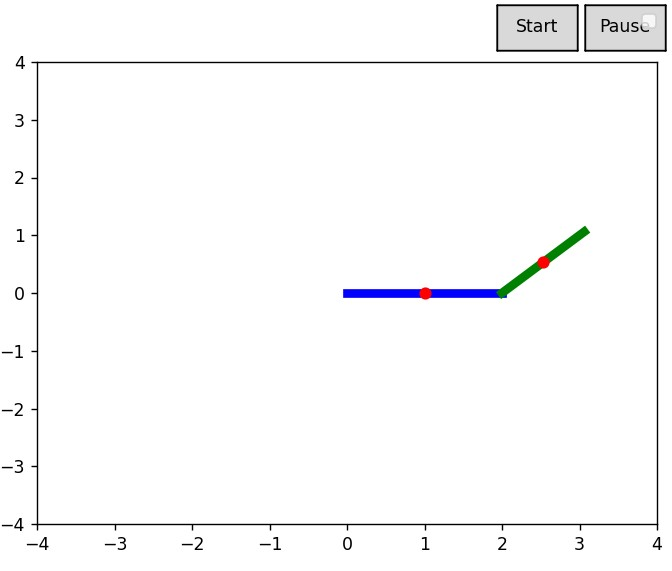
\includegraphics[width=0.5\linewidth]{latex_media/component_4_start of propagate arm.jpg}
    \caption{start of propagate arm}
    \label{fig:12}
\end{figure}

\begin{figure} [H]
    \centering
    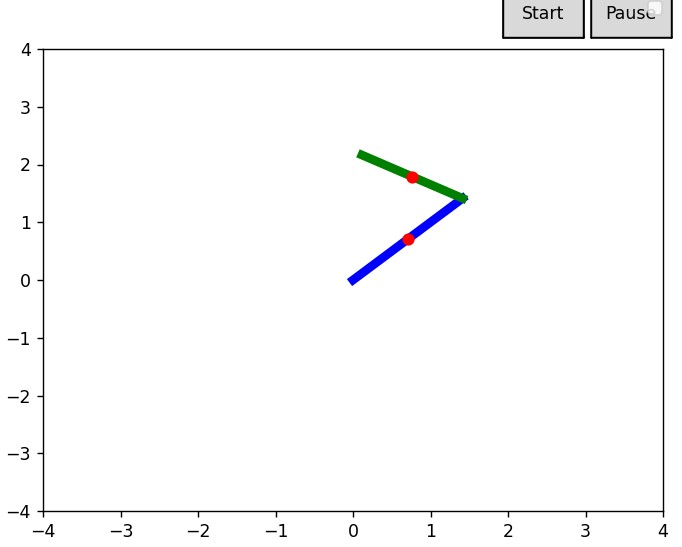
\includegraphics[width=0.5\linewidth]{latex_media/component_4_middle of propagate arm.jpg}
    \caption{middle of propagate arm}
    \label{fig:13}
\end{figure}

\begin{figure} [H]
    \centering
    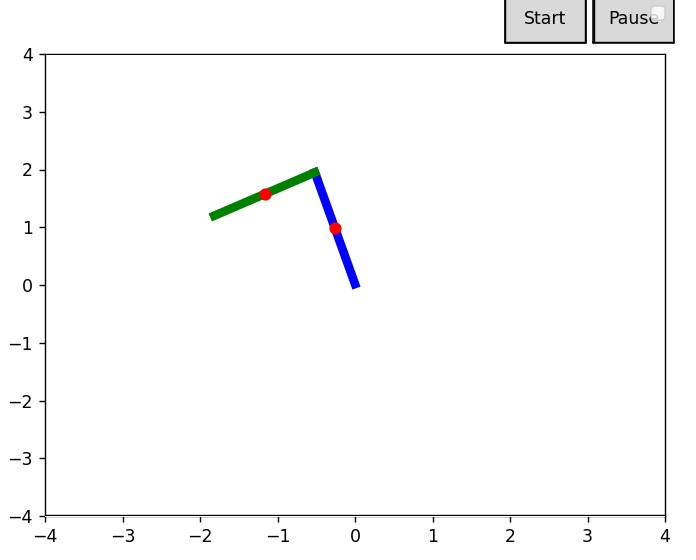
\includegraphics[width=0.5\linewidth]{latex_media/component_4_end of propagate arm.jpg}
    \caption{end of propagate arm}
    \label{fig:14}
\end{figure}

\subsection{\texttt{visualize\_arm\_path(path)}}

This function was similar to the last problem's animation to view the path of the two-link arm robot this time. It uses Matplotlib's library to help. For the plotting, we need the joint position and center of the link for each part of the arm. In the function, it is $c_{x}$, $c_{y}$ for the center of the link and x, y for the joint point. We update based on the pose that is sent from the path and then add it to the initial set for plotting. After we use some built in libraries from Matplotlib for animating, and start and pause functionality. (Gifs in folder)

\end{document}